%%% Local Variables: 
%%% mode: latex
%%% TeX-master: t
%%% End: 

\section{Data Structures} \label{ss:datascructures}
\subsection{Introduction}
The data flows and data structures used in the application are the interface between the functional blocks. A clear definition of the data will allow sharing the workload between different groups without causing too much communication overhead. The data structures are part of the \textbf{Data Dictionary}.

Data can be distinguished in data storage which is remembered as a system state: “data stored on-board” see SUBSET-026-A.3.4, and data temporarily stored.


Data structures shall be designed for:

\FIXME{API Synchronization}
Inputs (to be synchronised with the API specification):
\begin{itemize}
\item structures for messages
\item data from other inputs: odometer, DMI, TIU, STM's
\end{itemize}

\FIXME{API Synchronization}
Outputs (to be synchronised with the API specification):
\begin{itemize}
\item structures for output messages
\item data to other outputs: DMI, TIU/BIU, STM's, JRU (not including technical communication, like distributing the system time)
\end{itemize}


\subsection{Data structures to store received messages}
Messages are received either by Euroradio or Eurobalise (Euroloop is not yet taken into account). The Euroradio will provide a message in one block of data, from a Eurobalise Telegrams (the part of a message sent by one balise) are received, which have to be put together into a message.

Eurobalise Messages contain a header to give the following information:
\FIXME{Needs synchronization according to SUBSET-026-8.4.2.1}
\begin{itemize}
\item valid version of ERTMS/ETCS system
\item \verb+NID_BG+ identifier of the BG 
\item \verb+NID_C+ identifier of the country
\item reference to which information is given (identifier of the LRBG), in case of a radio message.
\item information for constructing the message out of the Telegrams and for checking message consistency (balise numbering, message counter, duplicate information etc.)
\end{itemize}

Euroradio Messages contain a header to give the following information:
\FIXME{Needs synchronization according to SUBSET-026-8.4.4.6.1}
\begin{itemize}

\item \verb+NID_MESSAGE+ - identifying the message number
\item \verb+L_MESSAGE+ - Message length including everything from field 1 to padding inclusive
\item \verb+T_TRAIN+ - Time Stamp from RBC
\item \verb+M_ACK+ - Inidicating of the message must be acknowledged
\item \verb+NID_LRBG+ - identifying the  
\item further variables as required by \verb+NID_MESSAGE+
\end{itemize}

The message header is used to check the consistency, to check if the message is valid for the current direction, define the reference for location based data and construct the message out of Telegrams.

Further messages contain “packets” as defined in SUBSET-026 chapter 7. 

Radio-messages are received as a bit stream in a minimised data format. To allow efficient processing the data has to stored using standard data-types (fixed point) in structures for individual packets. The chain of components between receiving the message from the antenna to storing packets using standard types is:
\FIXME{needs a design decision - consistent with high level architecture?}
radio - EVC basic software – bit walker – filtering.
Functions are assigned as follows to the different modules and functional blocks:
\begin{itemize}
\item CRC checking shall be done in the radio. The result of the CRC check shall be made available for the application software.
\FIXME{Exact definition of CRC error needs to be added here} (because a CRC error is to handled by the application as a consistency error, i.e. “linking reaction”).
\item Translating the bit stream into variables of a standard (fixed point) data-type and store the data in a memory accessible by the application software. The way the data stream has to be put into variables and stored depends on the version of the track-side ETCS installation. (see \verb+M_VERSION+ and SUBSET-026-6)
Indexes (``pointers'') shall be set to packets contained in the message, i.e. an array containing  the indexes of the first packet of a certain type. The array shall have one element per possible packet. Each packet shall have an extra field to refer to the next packet of the same type in the message (only possible for a few packet types).
This shall be done by the “bit walker”.
\item Detecting the version of the track-side ETCS system is to be handled in the application.
\item Check on illegal values in the packets. (if detected, set a flag for “consistency error”).
\item Couple the location reference to the different packets (those can be different for different packets in case infill information is included in the message, i.e. all packets after packet 136 contain infill information (have to be reference to the LRBG using linking information).
\item Translate the identity of the location reference (a BG) from \verb+NID_BG+ to the index and array where the concerning information is stored.
\item Check if the packets have to be taken into account or have to be stored in a transition buffer according to the current mode and level (filtering) and mark the packets if they shall be used.
\end{itemize}

To facilitate the above described functions, a data structure is necessary capable of storing at least 2 complete messages plus extra variables to store the result of CRC checking and the check on illegal values. Further for each packet variables are needed to store the reference position for the information in the packet (\verb+NID_BG+ and index plus array where the BG information is stored). In addition an array is needed to store “pointers” to the start of each packet in the message.



\begin{figure}[ht]
\centering
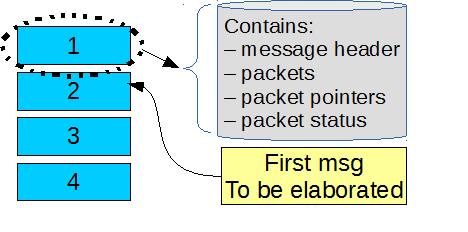
\includegraphics[scale=0.6]{../images/DataStructure_NotYetElaboratedMessages.png}
\caption{Data structure to store not yet elaborated messages.}\label{fig:DataStructureTelegramStructure}
\end{figure}


Data structure to store not yet elaborated messages as found in figure \ref{fig:DataStructureTelegramStructure} are further described in \ref{fig:SingleElementLocationBasedDataStructure} and \ref{fig:SingleElementLocationBasedDataStructure}. A special value for the ``pointer'' is defined for the case no radio messages are available.
Further pointers to the individual packets are required for efficient elaboration later on. 

The different functions can work on the same data structure, i.e. the structure is filled once and is than used up to the point where the packets are elaborated.


Eurobalise (BTM) -messages are received as a bit stream in a minimised data format per balise telegram. To allow efficient processing the data has to be stored using standard data-types (fixed point) in structures for individual packets. The chain of components between receiving the message from the antenna to storing packets using standard types is:
BTM - EVC basic software – bit walker – filtering.

\FIXME{needs a design decision - chain of components consistent with high level architecture?}
Functions are assigned as follows to the different modules and functional blocks:
\FIXME{CRC checking to be better described}
\begin{itemize}
\item CRC checking shall be done in the BTM per Telegram. The result of the CRC check shall be made available for the application software (because a CRC error is to handled by the application as a consistency error, i.e. “linking reaction”).
\item Translating the bit stream into variables of a standard (fixed point) data-type and store the data in a memory accessible by the application software . If there is already a Telegram from the same balise stored and depending on the message counter of the telegram header, the new data shall overwrite that Telegram. The way the data has to be stored depends on the version of the track-side ETCS installation.
\item “Pointers” shall be set to packets contained in the message, i.e. an array containing  the indexes of the first packet of a certain type. The array shall have one element per possible packet. Each packet shall have an extra field to refer to the next packet of the same type in the message (only possible for a few packet types).
This shall be done by the “bit walker”.
\item Detect the version of the track-side ETCS system, to be done in the application.
\item Check on illegal values in the packets. (if detected, set a flag for “consistency error”).
\item Couple the location reference to the different packets (those can be different for different packets in case infill information is included in the message, i.e. all packets after packet 136 contain infill information.
\item Compose a message out of the Telegrams if a balise of another BG is found, if all balises of a BG are found, if the maximum distance (12m) since the last detected balise has been passed.
\item Gather the BG information needed to build the “reference (coordinate) system”.
\item Translate the identity of the location reference (a BG) from \verb+NID_BG+ to the index and array where the concerning information is stored, see figure \ref{fig:DataStructureLocationBasedData}.
\item Check if the packets have to be taken into account or have to be stored in a transition buffer according to the current mode and level (filtering) and mark the packets if they shall be used.
\end{itemize}

\FIXME{what is the rationale behind only storing 15 telegrams?}

To facilitate the above described functions, a data structure is necessary capable of storing at least 15 telegrams plus extra variables to store the result of CRC checking and the check on illegal values. Indexes (“pointers”) indicating where the information of a completed message can be found shall be set. BG information (location, the identity of the BG, etc.) has to be stored in a separate structure for further evaluation. Further for each packet variables are needed to store the reference position for the information in the packet (\verb+NID_BG+ and index plus array where the BG information is stored). In addition an array is needed to store “pointers” to the start of each packet in the message.


\begin{figure}[ht]
\centering
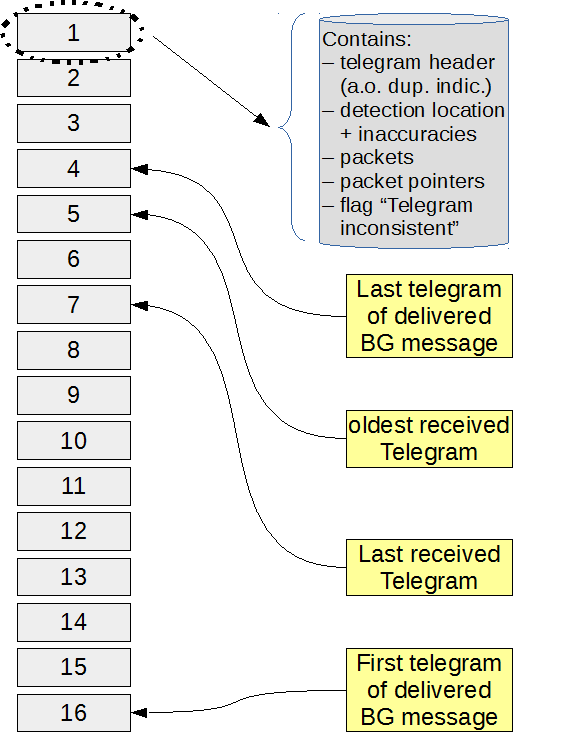
\includegraphics[scale=0.6]{../images/DataStructure_TelegramStructure.png}
\caption{“Telegram structure”: Structure in which Telegrams shall be stored by the “bit walker”.}\label{fig:DataStructureTelegramStructure}
\end{figure}



A completed message can during the consistency check and the check on linking, be kept in the same structure.

In the example shown in figure \ref{fig:DataStructureTelegramStructure}:
\begin{itemize}
\item A message is just made available consisting of 5 telegrams stored at position 16, 1,..,4.
If no message is available the pointers \textbf{``last telegram of delivered BG message''} and \textbf{``First telegram of delivered BG message''} message have a special value. After elaboration of the message and retrieving the packets (done in the same cycle) the pointers will be reset to this special value
\item Since receiving the last Telegram of the delivered message, 3 more (5, 6, 7) Telegrams were detected.
\item \textbf{“Oldest received Telegram”}: the oldest Telegram stored by the “bit walker” which has not been used in a completed message. If no Telegram is waiting for the completion of a BG-message the “pointer” shall have a special value.
\item \textbf{“Last received Telegram”}: the last Telegram stored by the “bit walker”. If no Telegram is waiting for the completion of a BG-message the “pointer” shall have a special value.
\end{itemize}


For packages which are not yet to be taken into account a data structure has to be designed to store the packages for later use inside the \textbf{``transition buffer''}. The stored packages shall be elaborated if the mode and level for which they are stored is reached (generic condition or shall those be stored with the packet).
The minimum number of packages which could have to be remembered, i.e. the minimum storage capacity to be reserved, is to be determined.
\FIXME{determine minimum packages to be remembered within the transition buffer}

\subsection{Data structures to store input data from other sources}

Other input data:
\begin{itemize}
\item TIU: Isolation, brake status (commanded, pressure, inhibited,...)
\FIXME{to be completed}
\item DMI: data-entry, acknowledgements, etc. 
\FIXME{to be completed}
\item STM's: out of scope for the current project. 
\end{itemize}

TIU
The data coming from the TIU is wrapped up in SUBSET-034 and needs amendments for the specific use of the OBU inside a locomotive. A data structure for storing all possible information shall be designed.
\FIXME{complete design of TIU related  data}

DMI
The data coming from the DMI, consists of inputs required based on information sent to the DMI in the context of a procedure.



\subsection{Data structures for “data stored on-board”}
This section is independent to the fact that what happens if the OBU is switched off
\FIXME{data stored on board needs to be completed}
\begin{enumerate}
\item Location based data (a.o. announced BG's, SSP, speed restrictions, location based level transitions, text messages,..)
\item Actual MRSP and list of targets as a distance from the trains front end. (taking into account the train length for speed increases if and where necessary).
\item Train Position
\item Reference (Coordinate) system 
\item announced BG's
\item Direct orders 
\item Intermediate analysis results (linking error, number of missed BG's, intervention curve passed,......)
\item BG lists for shunting and staff responsible
\item Train data
\item Data describing national rules (national and default values)
\item track data:  version, level priority
\FIXME{to differentiate the difference between track data and location based data}
\item Driver ID
\item Procedure status information (technical procedures and driver interactions)
\item Parameters tuning procedures (MA request parameters, Train position report parameters,....)
\item System mode and level
\item System status (including time to last self test)
\end{enumerate}
Below the types of data listed above are further described.


\subsubsection{Location based data}
In general “Location based data” is data giving a specific type of information related to a location on the track. Requirements concerning storing:
\begin{itemize}
\item  The reserved space shall be sufficient to store the maximum number of elements.
\item The elements shall be stored in the order they are passed on the track.
\item The location shall be available as a distance from the LRBG.
\end{itemize}
The minimum number of elements for which space shall be available is given in chapter \ref{sss:functionaldatastructure}, “Management of location based data”. For all types of location based data the same basis structure can be used, except for the location based information which can only contain one element (level transition order (LTO), reversing area, platform conditions, current limitation). The structure is described in chapter \ref{sss:functionaldatastructure}, “Management of location based data”:



\begin{figure}[ht]
\centering
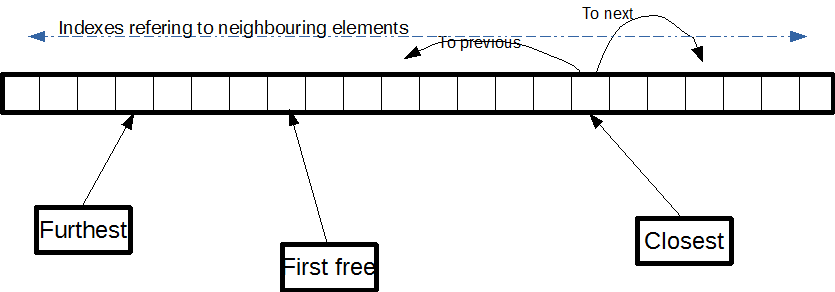
\includegraphics[scale=0.6]{../images/indexing_of_ringbuffer.png}
\caption{Data structure of ``location based data''}\label{fig:DataStructureLocationBasedData}
\end{figure}

\begin{figure}[ht]
\centering
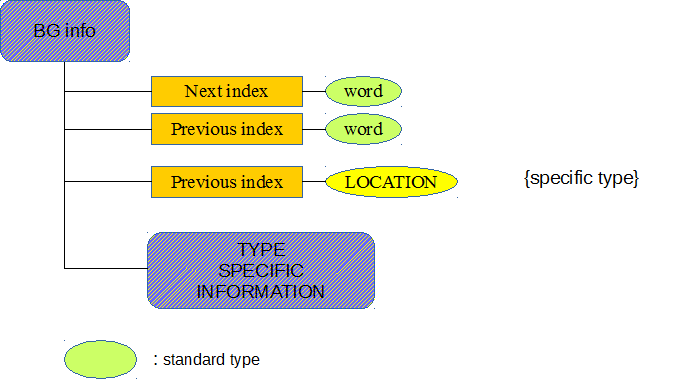
\includegraphics[scale=0.6]{../images/location_based_datastructure.png}
\caption{Single Element of data structure of ``location based data'' including backwards linking.}\label{fig:SingleElementLocationBasedDataStructure}
\end{figure}


\textbf{Actual MRSP and list of targets}
As described in chapter \ref{sss:functionaldatastructure} the MRSP and list of most restrictive targets is not stored as location based data, but as a set of distances with related speed level from the train front end. The rationale behind this is the ability to recalculate the MRSP when a restriction is revised.
At figure \ref{fig:SingleElementLocationBasedDataStructure} the structure of one element of the MRSP or list of targets is shown graphically.

\begin{figure}[ht]
\centering
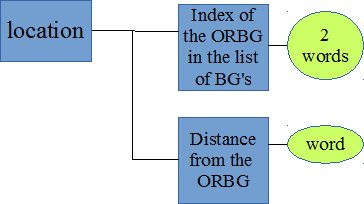
\includegraphics[scale=0.6]{../images/ORBG.png}
\caption{MRSP element as dependant from distance to target and further conditions}\label{fig:SingleElementLocationBasedDataStructure}
\end{figure}
\FIXME{Mode is also a condition, better list all conditions or write ``Further conditions''}
\FIXME{explain BCM}

The elements shall be stored in the order in which they are passed. At each cycle the structure shall be update according to the distance driven. As for speed increases the maximum distance and for speed decreases the minimum distance is valid, the order of the elements in the MRSP may change during driving from the LRBG.


\subsubsection{Train Position}
The train position shall be available for the train's safe front end, the safe rear end in case train integrity is used and the active antenna as a minimum, estimated and maximum distance from the nominal position of the LRBG:

\begin{center}
\begin{tabular}{ l || c | c | c }
  -       & Minimum & Estimated & Maximum \\ \hline \hline
  front  & X & X & X \\ \hline
  rear   & O & O & O \\ \hline
  antenna& X & X & X \\ \hline 
\multicolumn{4}{l}{X - mandatory} \\
\multicolumn{4}{l}{O - optional in case train integrity is used} \\
\end{tabular}
\captionof{table}{Availability of safe distances}\label{tbl:AvailableSafeDistances}
\end{center}


To be able to retrieve this data the following data is stored:
\begin{itemize}
\item The measured distance (raw data from the odometer) stored as a passing location (of the active antenna) for the LRBG 
(to be stored in the structure of the “list of passed BG's”).
\item The passing direction of the LRBG (nominal or reverse): for reporting to the RBC.
(to be stored in the structure of the “list of passed BG's”).
\item The antenna (A or B side in case a second antenna in installed) which reads the LRBG 
(to be stored in the structure of the “list of passed BG's”)
\item The distance between the antenna A and front end of cab A (cab A)
\item The inaccuracy in the distance between the antenna A and cab A (installation inaccuracy only)
\item The distance between the antenna A and cab B (installation inaccuracy only)
\item The inaccuracy in the distance between the antenna A and cab B
\item The distance between the antenna B and cab A
\item The inaccuracy in the distance between the antenna B and cab A (installation inaccuracy only)
\item The distance between the antenna B and cab B (installation inaccuracy only)
\item The inaccuracy in the distance between the antenna B and cab B
\end{itemize}

Together with the inputs “actual train position” and the “train orientation”,  all combinations given in the table above can be generated.


\subsubsection{Reference (Coordinate) system}
\FIXME{for the correction distance a design decision is needed and additional justification since this is not part of the SRS - relates to the complete subsubsection ``Reference (Coordinate) System)}
The data stored shall allow to calculate the distance between the train and a track-side element whose location is given as a distance from the nominal position of any BG. Therefore data shall be available concerning the relation between the distance from the nominal position of the LRBG and the distance from the nominal position of any other BG (further called ORBG), see figure \ref{fig:SingleElementLocationBasedDataStructure}. This distance is further called the “correction distance” and is BG specific. Therefore is shall be stored in the data structure for detected and announced BG's.
This “correction distance” can be derived from linking (exact) or from odometer data (with a tolerance). Further the possible distance between the position where a BG is detected and it's nominal position is to be taken into account.

\begin{figure}[ht]
\centering
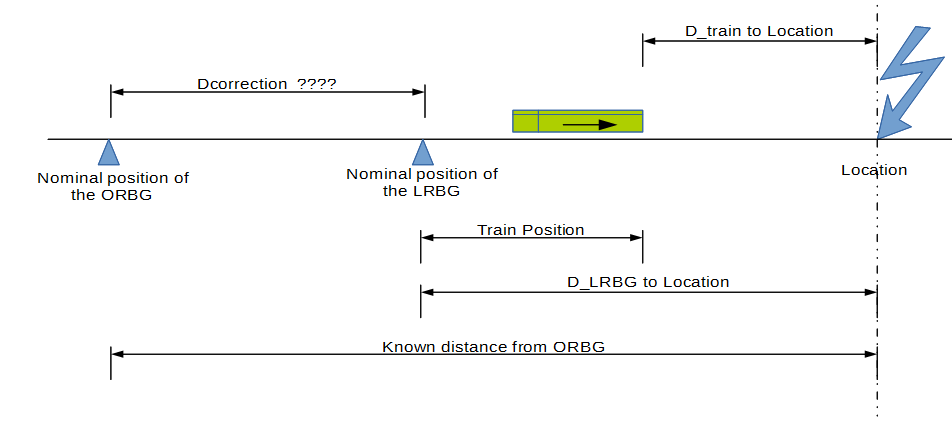
\includegraphics[scale=0.6]{../images/DataStructure_ReferenceSystem_CorrectionDistance.png}
\caption{Calculation of the distance from the train to an a track-side element (“Location”)}\label{fig:ReferenceSystemForCorrection}
\end{figure}
\FIXME{for this principle a justification and design decision is needed}

Therefore for each BG already passed, in reference to which the location of any track-side element is given a minimum and maximum correction distance shall be stored in order to be able to calculate the minimum and maximum distance between the train front end and the track-side element: 

Distance between train and location =
Distance from ORBG – Train Position (I.r.t. LRBG)  -  the stored correction distance (all including tolerances).


As the Location of a track-side element can also be given in reference to a BG in advance of the train (infill information), the same correction distance shall be available for announced BG's. This is only with one difference. For announced BG the exact linking distance is available (if not the infill information can and must not be taken into account). The correction distance exact (no minimum and maximum), and equal to the linking distance.

This leads to the need for two data structures, one storing the correction distances for already passed BG's, and one storing the announced (linking) distance from the nominal position of the LRBG to the announced BG's. The latter structure also contains the data needed for checking the linking consistency, i.e. the expectation window. A graphical representation of the data structure is given below: 

\begin{figure}[ht]
\centering
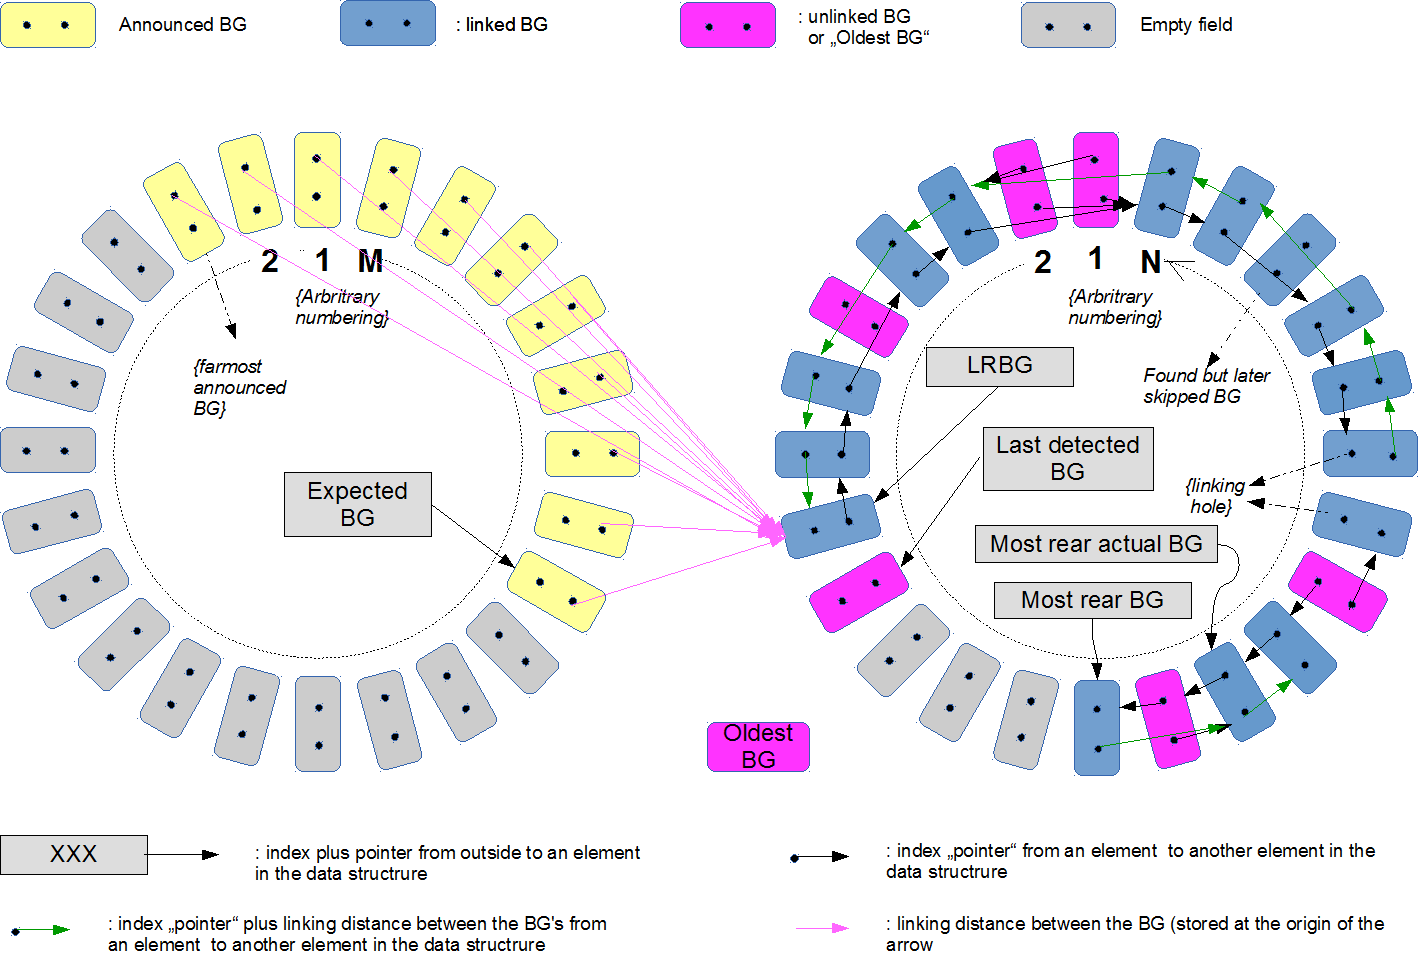
\includegraphics[scale=0.4]{../images/DataStructure_Linking.png}
\caption{Data structures for announced,  detected linked and detected unlinked BG's}\label{fig:DataStructureLinking}
\end{figure}

\FIXME{for this principle a justification and design decision is needed}



\begin{enumerate}
\item LRBG: “last relevant BG” = the last detected linked BG
\item Last detected BG: can be different from the LRBG if the last detected BG is marked as “unlinked”
\item Most rear actual BG:  most rear BG to which one or more “Locations” refer as being their ORBG ( original reference BG). All BG's more in rear may be deleted from the list.
\item Most rear BG: the most rear BG whose information is still stored in the “list of detected BG's”
\item “Oldest BG”: BG to which all “Locations” with an ORBG in rear of the “most rear BG” refer. This is used if the “List of detected BG's” is full. Between the “oldest BG” and the “most rear BG” no linking distance is available. Therefore the accuracy for the concerned locations will decrease.
linking hole: Number of linked BG's for which no linking information is available (see figure xx).
skipped BG: Linked BG which was detected when no BG's were announced, but which is not included in linking information received after wards (see figure xx)
“pointer”:  index of the element in the data structure where is referred to.
\end{enumerate}

\subsubsection{Direct orders}
Direct orders can be given for several actions, e.g. command the service or emergency brake, “stop if in staff responsible” etc. Direct orders which have immediate effect at the first evaluation like direct level and mode transitions (have immediate effect in the functional block “filtering” because they shall be taken into account at filtering further information in the message) can be rejected. 
Direct orders shall be stored in the internal data structure to allow the correct execution of the order by the concerning functional block. For each possible order a field shall be reserved, i.e. an array with a field for every possible order shall be build.

This data structure is needed to avoid getting event driven software, as the orders are stored and read by the a functional block which is commanded cyclically.
Direct orders to be stored (as a flag or variable):
\begin{itemize}
\item command service brake
\item “stop in staff responsible”
\item SR authorisation
\item Exit of trip mode
\item Inhibition of revoking TRS's
\end{itemize}
\FIXME{List needs to be completed by all orders including a special value ``now'' according to SUBSET-026-7}

\FIXME{ To what extent shall mode changes following from input data be taken into account before filtering?}

Intermediate analysis results (linking error, nb of missed BG's, intervention curve passed,......)
Just like direct orders, some analysis results shall lead to a certain specified action. For example, having a consistency error shall lead to the linking reaction (given from track-side or the default value which is command service brake). Just like direct orders those intermediate results are stored as an order for other functional blocks, in stead of immediately (event driven) calling the specific function.
Intermediate results to be stored (as a flag or variable):
\begin{itemize}
\item From BCM: EB intervention, SB intervention, acoustical warning, Vsoll, Vwarning,...
\item From linking consistency checking: type of linking reaction, number of missed BG's
\item From message consistency checking: type of linking reaction
…...
\FIXME{needs to be completed}
\end{itemize}

\subsubsection{BG lists for shunting and staff responsible}
Together with the order to go to shunting or to staff responsible a list of BG's which may be passed can be given. Both sets need to be storable in parallel.
The data structure shall consist of an array storing the identities of the BG's which may be passed. As the passing order is not always predictable it doesn't make sense to reorder them. BG's may thus be stored in the same order as they were received.


\subsubsection{Data describing the train } \label{sss:datadescribingthetrain}
To allow the usage of the system on all different train types, data describing the specific train shall be stored. The source of the data can be the TIU, the data entry unit or default values. Data to be stored includes:
\begin{itemize}
\item Train category(-ies)
\item Train length
\item Traction / brake parameters
\item Maximum train speed
\item Loading gauge
\item Axle load category
\item Traction system(s) accepted by the engine
\item Train fitted with airtight system
\item List of National Systems available on-board
\item Number of axles
\end{itemize}
Each parameter shall have a flag to indicate if this parameter can be edited by the driver.
Each parameter shall have a flag to indicate if this parameter can be displayed on demand by the driver.


\subsubsection{Data describing national ruling}
Maximum speeds, braking curve margins, roll away distance, timing for certain conditions, procedural information etc. may differ from country to country.
Therefore a list of national values is defined according to SUBSET-026-A3.2. These national values shall be stored on board, to be available for all functional blocks. 

For those national values, defaults can be defined for the case no national values have been received from track-side. A similar structure shall be provided to remember those default values.


\subsubsection{Track Data}
The version of the track-side ETCS system and the priority of levels supported from track-side shall be available for the functional blocks. Data structures to store this information in the same format as it is received from track-side shall be provided.


\subsubsection{Driver Data}
Driver data is used when displaying data to the driver (language) and for juridical recording (driver ID). A data structure shall be defined to store all possibly available driver data, see also chapter \ref{sss:datadescribingthetrain}


\subsubsection{Procedure status information}
In the SRS (especially SUBSET-026 chapter 5) a number of procedures between track-side, train and driver are described, e.g.
\begin{itemize}
\item data-entry
\item reporting train position
\item SoM, EoM
\item override
\item Train data management....
\item text message acknowledgements
\item establishing and ending a connection to the RBC
\item RBC-RBC hand over
\item transition to shunting
\item transition to staff responsible
\item …...
\item \FIXME{complete procedure}
\end{itemize}

For each of these procedures the status shall be remembered, in some cases including the time since specific events.
Therefore for each procedure a global data structure shall be designed to remember the status of each procedure.


\subsubsection{Parameters for procedures}
As the requirements concerning procedures may differ, parameters are defined to tune the procedures. (timing requirements, etc.). Data structures to store this information in the same format as it is received from track-side shall be provided.


\subsubsection{System mode and level}
The system mode and level shall be available to all functional blocks at any time. Therefore variables to store the current state and level shall be defined.


\subsubsection{System status}
Data structures are necessary to store the current status of the subsystems (Radio, BTM, LTM, STM, JRU, odometer, TIU, brakes). 


\subsubsection{Data structures to store messages to be sent to the RBC}
The information needed which as to be sent to the RBC is provided by “train supervision”, “mode/level management”, diverse procedures etc. 
To sent them to the RBC the information has to be build in a specific format (specified in ss026, chapter 7 and 8). This structure has to be synchronised with the API specification


\subsubsection{Data structures to sent to subsystems (DMI, TIU/BIU, JRU, STM)}
Information to be sent to the DMI and TIU/BIU shall be build in data structures as described in the API specification.
The JRU and STM are out of scope for the current iteration.

